% Chapter 9: Causal Inference and Reinforcement Learning
% Formalizes confounded MDPs, presents backdoor-adjusted OPE,
% and demonstrates via simulation.
%
% NOTE: Terminology convention for this chapter. "Outcome" is used ONLY when
% referring to the causal inference concept Y (potential outcome in Rubin's
% framework, or endogenous variable in Pearl's SCM). In the RL/MDP framework,
% the corresponding quantities are: reward R_t, next state S_{t+1}, return
% G_t, or value V^\pi. When mapping between frameworks, always specify which
% framework's vocabulary is being used. See the footnote on the first use of
% "reward or state transition" for the reader-facing version of this convention.

Reinforcement learning algorithms solve Markov decision processes by estimating value functions or optimizing policies from sampled transitions. Two assumptions underlie the standard formulation. First, the agent's action at time $t$ is determined solely by the observed state $s_t$ and the agent's policy $\pi(a \mid s_t)$; there is no unobserved variable (confounder) simultaneously influencing both the action and the reward or state transition.\footnote{In causal inference, ``outcome'' refers specifically to the response variable $Y$ (or the potential outcome $Y(d)$ in the Rubin framework). The RL/MDP framework has no single corresponding concept called ``outcome''; the relevant quantities are the reward $R_t$, the next state $S_{t+1}$, the return $G_t = \sum_{k=0}^\infty \gamma^k R_{t+k}$, or the value function $V^\pi(s)$. When economists refer to the ``outcome model'' $\mathbb{E}[Y \mid X, D]$, the RL analogue is the action-value function $Q(s,a)$. Throughout this chapter, I reserve ``outcome'' for its causal inference meaning and use the specific RL quantity (reward, state, return, value) elsewhere.}
% NOTE: "outcome" replaced with "reward or state transition" — the two RL quantities
% that a confounder can distort. The footnote establishes the cross-framework
% terminology convention that governs the rest of the chapter.
Second, the observed state $s_t$ is sufficient for prediction, so that conditioning on $s_t$ renders future states independent of past history. Both assumptions are the Markov property restated in causal language. Both fail routinely in economic applications.

The preceding chapters operated under a third assumption that was so natural it required no mention: the analyst controls data collection. In the tabular algorithms of Section~\ref{section:rl_algorithms} and the gridworld study of Section~\ref{section:illustrated_example}, each method generated its own trajectories by executing actions in a simulator and observing the consequences. The bandit algorithms of Section~\ref{section:bandits} chose arms and observed payoffs in real time. Even when exploration was limited, the data-generating process was known because the agent's own policy produced it. This chapter drops that assumption entirely. The analyst receives a fixed log of decisions made by someone else, a behavioral policy $\mu$ whose functional form may be unknown and whose action choices may depend on variables the analyst cannot observe. The data are observational in the econometric sense: the analyst had no role in generating them and cannot rerun the experiment under a different policy. Identification, not optimization, becomes the central problem.

Unobserved demand shocks that affect both a retailer's pricing algorithm and consumer demand create endogeneity: the observed correlation between price and demand conflates the causal effect with the confounding effect. An RL agent trained on such observational data converges to a biased policy that systematically overestimates the revenue from high prices.

This chapter formalizes the confounded MDP, presents backdoor-adjusted off-policy evaluation as the key algorithmic solution, and demonstrates its practical consequences through a simulation study in a confounded chain MDP. For comprehensive surveys of the rapidly growing causal RL literature, including causal representation learning, counterfactual policy optimization, transfer, and fairness, I refer readers to \citet{deng2023causal} and \citet{dacostacunha2025unifying}.

%%%%%%%%%%%%%%%%%%%%%%%%%%%%%%%%%%%%%%%%%%%%%%%%%%%%%%%%%%%%%%%%%%%%%%%%%%%%%%%
\subsection{The Confounded MDP}
\label{subsec:confounded_mdp}
%%%%%%%%%%%%%%%%%%%%%%%%%%%%%%%%%%%%%%%%%%%%%%%%%%%%%%%%%%%%%%%%%%%%%%%%%%%%%%%

Standard MDPs assume that the state $s_t$ is fully observed and that the agent's policy depends only on $s_t$. In the online algorithms of earlier chapters, these assumptions held by construction: the agent executed its own policy in a known environment, so no unobserved variable could simultaneously influence action selection and transitions. When unobserved confounders influence both the behavioral policy and the transitions or rewards, the MDP is confounded. This formalization, developed by \citet{zhang2019near}, \citet{zhang2020causal}, and \citet{kallus2020confounding}, provides the foundation for causal reasoning in sequential decision problems. The key tool is Pearl's do-operator. The interventional distribution $P(Y \mid \operatorname{do}(X = x))$ is the distribution that arises when $X$ is set externally rather than observed passively, severing all incoming causal influences on $X$ while leaving the remaining data-generating process intact.\footnote{The do-operator is formalized within the structural causal model (SCM) framework of \citet{pearl2009causality}. An SCM specifies endogenous variables $\mathbf{V}$, exogenous variables $\mathbf{U}$, structural equations $V_i = f_i(\text{pa}(V_i), U_i)$, and a distribution $P(\mathbf{U})$. The intervention $\operatorname{do}(X = x)$ replaces the structural equation for $X$ with a constant, producing the interventional distribution. See \citet{pearl2009causality} for the complete framework, including the causal hierarchy (association, intervention, counterfactual) and general identification theory.}

% NOTE: Definition 1 is entirely in RL/MDP vocabulary. No causal inference terms
% appear here — the confounded MDP is an MDP augmented with unobserved variables.
\begin{definition}[Confounded MDP {\citep{zhang2020causal}}]
\label{def:confounded_mdp}
A confounded MDP is a tuple $(\mathcal{S}, \mathcal{A}, \mathcal{U}, P, r, \gamma)$ where $\mathcal{S}$ is a finite state space, $\mathcal{A}$ is a finite action space, $\mathcal{U}$ is a space of unobserved confounders, $\gamma \in [0,1)$ is a discount factor, and the dynamics are governed by structural equations:
\begin{align}
U_t &\sim P_U(\cdot \mid S_t), \label{eq:cmdp_confounder} \\
A_t &\sim \mu(\cdot \mid S_t, U_t), \label{eq:cmdp_action} \\
R_t &= f_R(S_t, A_t, U_t) + \epsilon_t, \label{eq:cmdp_reward} \\
S_{t+1} &\sim f_S(\cdot \mid S_t, A_t, U_t). \label{eq:cmdp_transition}
\end{align}
The behavioral (logging) policy $\mu$ depends on the unobserved confounder $U_t$ through Equation~\eqref{eq:cmdp_action}. An evaluation policy $\pi(a \mid s)$ depends only on the observed state.\footnote{A confounded MDP differs from a partially observed MDP (POMDP). In a POMDP, the agent knows its observation is incomplete and optimizes accordingly; the hidden state affects what the agent sees but the analyst models this explicitly. In a confounded MDP, the hidden variable $U_t$ distorts the behavioral policy $\mu$ without the analyst's knowledge or control, so the core challenge is not planning under partial observability but rather identifying interventional quantities from data generated by a policy that depended on variables the analyst cannot observe.}
\end{definition}

The separation between the behavioral policy $\mu$ and the evaluation policy $\pi$ is the formal signature of offline RL. In the online algorithms of Sections~\ref{section:rl_algorithms}--\ref{section:illustrated_example}, the behavior and target policies were identical (on-policy methods) or related by a known exploration mechanism ($\epsilon$-greedy, softmax); here, $\mu$ is an unknown function of unobserved variables.

The key distinction is between observational and interventional transition dynamics. Under the behavioral policy $\mu$, which depends on $U_t$, the conditional distribution $P(s' \mid s, a)$ obtained by conditioning on the observed action does not equal the interventional distribution obtained by setting the action externally:
\begin{equation}
P(s' \mid s, a) \neq P(s' \mid s, \operatorname{do}(a)).
\label{eq:obs_vs_interventional}
\end{equation}
The left-hand side conditions on the event $\{A_t = a\}$, which carries information about $U_t$ through the behavioral policy $\mu$. The right-hand side intervenes on $A_t$, severing the dependence between action and confounder. When $U_t$ also affects $S_{t+1}$ through Equation~\eqref{eq:cmdp_transition}, the conditioning introduces a spurious association between $a$ and $s'$.

The Bellman equation for policy evaluation must use interventional, not observational, transition probabilities. Define the causal Bellman operator for a target policy $\pi$:
% NOTE: The causal Bellman operator deliberately uses hybrid notation — Pearl's
% do-operator (causal inference) applied to RL quantities R_t, S_t, A_t. This is
% the point where the two frameworks formally merge; the do-operator modifies the
% standard Bellman recursion to use interventional rather than observational dynamics.
\begin{definition}[Causal Bellman Operator {\citep{zhang2020causal}}]
\label{def:causal_bellman}
The causal Bellman operator $\mathcal{T}_c^\pi$ for policy $\pi$ in a confounded MDP is
\begin{equation}
(\mathcal{T}_c^\pi V)(s) = \sum_{a \in \mathcal{A}} \pi(a \mid s) \sum_{s' \in \mathcal{S}} P(s' \mid s, \operatorname{do}(a)) \bigl[ r(s, a) + \gamma V(s') \bigr],
\label{eq:causal_bellman}
\end{equation}
where $r(s,a) = \mathbb{E}[R_t \mid S_t = s, \operatorname{do}(A_t = a)]$ is the interventional expected reward.
\end{definition}

When an analyst ignores confounding and uses the observational transition probabilities $P(s' \mid s, a)$ in place of $P(s' \mid s, \operatorname{do}(a))$, the resulting value estimates are biased.

\begin{lemma}[Bias of Naive Off-Policy Evaluation {\citep{kallus2020confounding}}]
\label{lem:naive_bias}
Let $\hat{V}^{\pi}_{\text{naive}}$ denote the value function obtained by solving the Bellman equation with observational transitions $P(s' \mid s, a)$, and let $V^\pi$ denote the true value function under interventional transitions $P(s' \mid s, \operatorname{do}(a))$. In a confounded MDP where $P(s' \mid s, a) \neq P(s' \mid s, \operatorname{do}(a))$ for some $(s, a, s')$, the naive estimator is biased:
\begin{equation}
\hat{V}^{\pi}_{\text{naive}}(s) \neq V^\pi(s).
\end{equation}
The importance-sampling estimator $\hat{V}^{\pi}_{\text{IS}} = \frac{1}{N} \sum_{i=1}^N \prod_{t=0}^{T} \frac{\pi(a_t^{(i)} \mid s_t^{(i)})}{\mu(a_t^{(i)} \mid s_t^{(i)})} G^{(i)}$, where $G^{(i)} = \sum_{t=0}^{T} \gamma^t R_t^{(i)}$ is the discounted return of trajectory $i$ and $T$ is the trajectory length, is also biased because the propensity $\mu(a \mid s)$ is not the true behavioral propensity $\mu(a \mid s, u)$.
\end{lemma}

The bias arises because the importance-sampling ratio $\pi(a \mid s) / \mu(a \mid s)$ does not correctly reweight the data. The true behavioral policy is $\mu(a \mid s, u)$, but since $u$ is unobserved, the analyst can only estimate the marginal propensity $\mu(a \mid s) = \mathbb{E}_{U}[\mu(a \mid s, U) \mid s]$. Reweighting by the marginal propensity does not eliminate the confounding bias.\footnote{This is the sequential analogue of the omitted variable bias in linear regression. In the static case, regressing $Y$ on $X$ without controlling for a confounder $U$ yields a biased coefficient. In the sequential case, the bias propagates through the Bellman recursion and can amplify over the horizon.}

The backdoor criterion \citep{pearl2009causality} provides a path to identification. \citet{zhang2020causal} apply it to the confounded MDP setting.

\begin{theorem}[Backdoor Identification in Confounded MDPs {\citep{pearl2009causality,zhang2020causal}}]
\label{thm:backdoor_mdp}
Suppose a set of observed variables $\mathbf{Z}_t$ satisfies the backdoor criterion relative to $(A_t, S_{t+1})$ in the causal graph of the confounded MDP, meaning that $\mathbf{Z}_t$ blocks all backdoor paths from $A_t$ to $S_{t+1}$ and no element of $\mathbf{Z}_t$ is a descendant of $A_t$.\footnote{A backdoor path from $A_t$ to $S_{t+1}$ is any path in the causal graph that begins with an arrow into $A_t$ (i.e., a non-causal path). In the confounded MDP, $A_t \leftarrow U_t \rightarrow S_{t+1}$ is a backdoor path: $U_t$ causes both $A_t$ and $S_{t+1}$, creating a spurious association. Blocking all such paths by conditioning on appropriate variables eliminates the confounding bias. See \citet{pearl2009causality}, Chapter~3.} Then the interventional transition probability is identified:
\begin{equation}
P(s' \mid s, \operatorname{do}(a)) = \sum_{\mathbf{z}} P(s' \mid s, a, \mathbf{z}) \, P(\mathbf{z} \mid s).
\label{eq:backdoor_mdp}
\end{equation}
Substituting Equation~\eqref{eq:backdoor_mdp} into the causal Bellman operator (Equation~\ref{eq:causal_bellman}) yields an identified, consistent estimator of $V^\pi$.\footnote{While Theorem~\ref{thm:backdoor_mdp} assumes $\mathbf{Z}_t$ blocks all backdoor paths, identification is also possible when $\mathbf{Z}_t$ are merely proxies (effects) of the unobserved confounder. This ``proximal'' approach to RL employs the theory of negative controls to recover interventional values without satisfying the backdoor criterion \citep{bennett2021proximal}.}
\end{theorem}

%%%%%%%%%%%%%%%%%%%%%%%%%%%%%%%%%%%%%%%%%%%%%%%%%%%%%%%%%%%%%%%%%%%%%%%%%%%%%%%
\subsection{Backdoor-Adjusted Off-Policy Evaluation}
\label{subsec:backdoor_ope}
%%%%%%%%%%%%%%%%%%%%%%%%%%%%%%%%%%%%%%%%%%%%%%%%%%%%%%%%%%%%%%%%%%%%%%%%%%%%%%%

% NOTE: This paragraph is the explicit framework mapping. It intentionally uses BOTH
% RL and causal inference vocabulary, since its purpose is to establish the correspondence.
% V^\pi (RL) <-> E[Y(d)] (Rubin). In the single-period case V^\pi reduces to
% E[R | do(a)] and Y(d) is the potential outcome under treatment d; the multi-period
% case involves discounted sums over the interventional trajectory distribution.
Off-policy evaluation under confounding is precisely an average treatment effect (ATE) estimation problem in a dynamic setting \citep{bannon2020causality}. The behavioral policy $\mu$ corresponds to the treatment assignment mechanism, the target policy $\pi$ to the counterfactual treatment regime, and the policy value $V^\pi$ to the expected potential outcome $\mathbb{E}[Y(d)]$ under the Rubin framework. Importance sampling in OPE corresponds to inverse probability weighting (IPW); doubly robust OPE corresponds to the augmented IPW (AIPW) estimator of \citet{robins1994estimation}. The key challenge, distribution shift between $\mu$ and $\pi$, is the analogue of the overlap (positivity) condition in causal inference.

In the online setting of earlier chapters, distribution shift did not arise: the data distribution tracked the current policy throughout training, so the state-action frequencies under which value estimates were formed matched the frequencies under which the policy would be deployed.

Theorem~\ref{thm:backdoor_mdp} yields a concrete estimation procedure. Given logged data $\{(s_t, a_t, z_t, r_t, s_{t+1})\}_{t=1}^N$ collected under behavioral policy $\mu$, where $z_t$ is an observed proxy for the confounder:
\begin{enumerate}
\item Estimate the conditional transition model $\hat{P}(s' \mid s, a, z)$ and the proxy distribution $\hat{P}(z \mid s)$ from the logged data.
\item Compute interventional transitions via the backdoor adjustment:
\begin{equation}
\hat{P}(s' \mid s, \operatorname{do}(a)) = \sum_{z} \hat{P}(s' \mid s, a, z) \, \hat{P}(z \mid s).
\label{eq:backdoor_estimator}
\end{equation}
\item Solve the causal Bellman equation (Definition~\ref{def:causal_bellman}) using the estimated interventional transitions to obtain $\hat{V}^\pi$.
\end{enumerate}
% NOTE: "outcome model" is the econometric term for E[Y | X, D]; the RL analogue is Q(s,a).
% We use RL vocabulary here since this paragraph describes the RL estimator, with
% the parenthetical bridging to the econometric name for readers from that tradition.
The doubly robust variant combines the fitted action-value function $\hat{Q}(s,a)$ (the RL analogue of the econometric outcome model) with backdoor-adjusted propensities, achieving consistency if either $\hat{Q}$ or the propensity model is correctly specified.

%%%%%%%%%%%%%%%%%%%%%%%%%%%%%%%%%%%%%%%%%%%%%%%%%%%%%%%%%%%%%%%%%%%%%%%%%%%%%%%
\subsection{The Broader Causal RL Landscape}
\label{subsec:causal_rl_landscape}
%%%%%%%%%%%%%%%%%%%%%%%%%%%%%%%%%%%%%%%%%%%%%%%%%%%%%%%%%%%%%%%%%%%%%%%%%%%%%%%

The confounded MDP and backdoor-adjusted OPE address one specific failure mode, but the intersection of causality and reinforcement learning extends considerably further. Three active research directions illustrate the scope.

Causal representation learning for RL seeks state representations $\phi(s)$ that capture causal mechanisms rather than spurious correlations. When superficial statistics change across environments but the underlying causal structure is preserved, policies learned on invariant causal features generalize where standard representations fail \citep{scholkopf2021toward}. \citet{dacostacunha2025unifying} formalize this as invariant policy optimization within a multi-environment MDP framework. Sim-to-real robotics illustrates the problem. A robot arm trained in a simulator with blue backgrounds and simple textures may learn to associate visual quirks with correct actions rather than learning the actual object positions that matter. When deployed on a real factory floor with different lighting, the policy fails. Training across multiple visually distinct simulators, same physics but different textures and lighting, forces the state representation to discard renderer-specific features and retain only causally relevant ones like object pose and joint angles \citep{dacostacunha2025unifying}.

Counterfactual policy optimization uses structural causal models to generate ``what-if'' trajectories for credit assignment and data augmentation. \citet{buesing2019woulda} introduce Gumbel-Max SCMs that produce counterfactual rollouts from a single observed trajectory, enabling off-policy evaluation without importance weights. This follows Pearl's Abduction-Action-Prediction procedure \citep{pearl2009causality}: first infer the exogenous noise $U$ that explains the observed trajectory (abduction), then replace the logged action with the counterfactual action (action), and finally propagate the modified action through the original structural equations to predict the counterfactual outcome (prediction). \citet{oberst2019counterfactual} extend this to Gumbel-Max SCM-based counterfactual off-policy estimation in healthcare settings, while \citet{forney2017counterfactual} demonstrate that counterfactual data-fusion can augment online RL exploration by generating synthetic transitions consistent with the learned causal model. In Atari Breakout, moving the paddle determines whether a brick breaks many timesteps later, but which of the dozens of intervening actions actually mattered? \citet{buesing2019woulda} answer this by replaying an observed trajectory with one action changed while holding the environment's random outcomes fixed. Because the real and counterfactual trajectories share the same randomness, any difference in reward is caused by that single action change, solving the long-horizon credit assignment problem without the compounding errors of model rollouts or the high variance of importance sampling.

Causal transfer in RL applies the transportability theory of \citet{pearl2014external} and \citet{bareinboim2016causal} to policy transfer across domains. Causal invariance identifies which components of a learned policy remain valid when the environment changes, enabling transfer in settings where standard domain adaptation, which relies on distributional similarity, fails because the intervention targets differ. Autonomous driving illustrates the advantage. A self-driving policy trained in simulation has access to millions of miles of data, but the simulator's graphics differ from real roads. Rather than treating this as one large distribution shift, selection diagrams identify which mechanisms are shared (physical dynamics of steering and braking) and which differ (visual rendering, weather effects) \citep{bareinboim2016causal}. The shared mechanisms transfer directly; only the differing components require recalibration with scarce real-world data.

For comprehensive surveys covering these directions and others, including fairness, safety, and partial observability, see \citet{deng2023causal} and \citet{dacostacunha2025unifying}.

%%%%%%%%%%%%%%%%%%%%%%%%%%%%%%%%%%%%%%%%%%%%%%%%%%%%%%%%%%%%%%%%%%%%%%%%%%%%%%%
\subsection{Alternative Identification Strategies}
\label{subsec:alternative_identification}
%%%%%%%%%%%%%%%%%%%%%%%%%%%%%%%%%%%%%%%%%%%%%%%%%%%%%%%%%%%%%%%%%%%%%%%%%%%%%%%

The backdoor criterion requires observing a variable $\mathbf{Z}_t$ that blocks all confounding paths. When no such variable is available, three alternative identification strategies apply, each with a direct econometric analogue.

When the backdoor criterion fails because confounders are unobserved, the front-door criterion offers an alternative if the action $A_t$ affects the next state $S_{t+1}$ only through an observed mediator $M_t$. The front-door criterion requires: (i) $A_t$ has no direct path to $S_{t+1}$ bypassing $M_t$, and (ii) no unblocked confounding between $M_t$ and $S_{t+1}$. When satisfied, a two-stage formula recovers the causal effect: first estimate how $A_t$ affects $M_t$, then how $M_t$ affects $S_{t+1}$ while adjusting for $A_t$ \citep{pearl2009causality}. This decomposition into direct and indirect effects is the sequential analogue of mediation analysis in econometrics \citep{dacostacunha2025unifying}.

The causal RL survey of \citet{dacostacunha2025unifying} illustrates the front-door criterion with a mobile wellness intervention. A health app (action $A_t$) aims to reduce patient cortisol levels (outcome $S_{t+1}$), but unobserved health consciousness $U_t$ confounds the relationship because health-conscious individuals are both more likely to adopt the app and more likely to have low cortisol regardless. The app affects cortisol only through an observed mediator, supplement adherence $M_t$. The front-door criterion exploits this structure in two stages. First, the effect of app usage on supplement adherence is unconfounded because health consciousness does not block the causal path from $A_t$ to $M_t$. Second, the effect of supplement adherence on cortisol is identified by adjusting for app usage, which satisfies the backdoor criterion for the $M_t \to S_{t+1}$ link. Combining these two estimates recovers the causal effect of the app on cortisol without ever observing health consciousness.

When neither backdoor nor front-door variables are available, instrumental variable methods can identify causal effects. An instrument $Z_t$ must satisfy two conditions: it affects the action $A_t$ (relevance) and its effect on $S_{t+1}$ is channeled entirely through $A_t$ (exclusion restriction). \citet{liao2024_iv_rl} formalize this as a Confounded MDP with Instrumental Variables (CMDP-IV), where transitions take the form $S_{t+1} = F^*(S_t, A_t) + \epsilon_t$ with unobserved confounders $\epsilon_t$ affecting both the behavior policy and transitions. Their IV-aided Value Iteration algorithm recovers the transition function $F^*$ from a conditional moment restriction $\mathbb{E}[F^*(S_t, A_t) \mid Z_t] = \mathbb{E}[S_{t+1} \mid Z_t]$, then runs standard value iteration on the estimated model.

\citet{liao2024_iv_rl} illustrate with neonatal intensive care unit (NICU) assignment. A hospital must decide whether to admit each newborn to the NICU (action $A_t$), and this decision is confounded by unobserved severity indicators that affect both the admission decision and the infant's health trajectory. Differential travel time from the hospital to a specialty care provider serves as an instrument $Z_t$. Relevance holds because longer travel times discourage NICU referrals, shifting the admission probability. The exclusion restriction holds because travel time affects infant health outcomes only through the admission decision, not directly. The conditional moment restriction $\mathbb{E}[F^*(S_t, A_t) \mid Z_t] = \mathbb{E}[S_{t+1} \mid Z_t]$ uses variation in travel time across hospitals to trace out the causal effect of NICU admission on health transitions, recovering the transition function $F^*$ that standard regression conflates with the unobserved confounder.

When confounders are truly latent but proxy variables, noisy correlates of the confounder, are available, proximal causal inference provides identification. \citet{bennett2021proximal} adapt this to sequential settings. The analyst observes two proxies: a treatment-side proxy $Z_t$ (e.g., previous observation $O_{t-1}$) and an outcome-side proxy $W_t$ (e.g., current observation $O_t$), both conditionally independent given the latent confounder $U_t$. Two bridge functions, analogous to inverse propensity scores and Q-functions, are estimated from data by solving conditional moment equations, yielding a doubly robust estimator of the policy value that is $\sqrt{n}$-consistent without ever observing $U_t$. \citet{bennett2021proximal} demonstrate with a sepsis management simulator in which physicians choose among fluids, vasopressors, and antibiotics at each decision point. The patient's diabetes status is the latent confounder, partially censored in the medical record so that 20\% of diabetic patients appear as non-diabetic in the data. Because the physician observes the true diabetes status when prescribing but the analyst's dataset contains the censored version, the behavioral policy depends on a variable the analyst cannot fully recover. Previous clinical observations $O_{t-1}$ (prior lab values and vitals) serve as the treatment-side proxy $Z_t$ because they correlate with diabetes status and influence the physician's current prescribing. Current clinical observations $O_t$ serve as the outcome-side proxy $W_t$ because they reflect diabetes status and predict future health transitions. In their experiments, the proximal estimator correctly identified which evaluation policy improved over the behavioral policy in 82--100\% of test cases, while naive estimators that ignored confounding and standard MDP estimators that assumed full observability both achieved 0\% accuracy.

%%%%%%%%%%%%%%%%%%%%%%%%%%%%%%%%%%%%%%%%%%%%%%%%%%%%%%%%%%%%%%%%%%%%%%%%%%%%%%%
\subsection{Simulation Study: Confounded Off-Policy Evaluation}
\label{subsec:sim_confounded_ope}
%%%%%%%%%%%%%%%%%%%%%%%%%%%%%%%%%%%%%%%%%%%%%%%%%%%%%%%%%%%%%%%%%%%%%%%%%%%%%%%

Unlike the simulations in Sections~\ref{section:illustrated_example}--\ref{section:applications}, where each algorithm generated its own training data through interaction, the estimators here receive a fixed dataset collected under the behavioral policy $\mu$. I construct a 5-state chain MDP $\mathcal{S} = \{0,1,2,3,4\}$ with two actions (advance, stay) and an absorbing goal at state 4. The causal structure at each step is $Z_t \to U_t \to A_t$ and $Z_t \to S_{t+1}$, where $Z_t \in \{0,1\}$ is an observed covariate drawn i.i.d.\ with $P(Z_t{=}1) = 0.5$, and $U_t \in \{0,1\}$ is an unobserved confounder with $P(U_t{=}1 \mid Z_t{=}1) = 0.9$ and $P(U_t{=}1 \mid Z_t{=}0) = 0.1$. Transitions depend on $Z_t$, not $U_t$: the advance action succeeds with probability $0.9$ when $Z_t = 1$ and $0.5$ when $Z_t = 0$; the stay action is a deterministic self-loop. Rewards are a deterministic step cost $r(s,a) = -1$ for $s < 4$, with $\gamma = 0.9$. The behavioral policy depends on the unobserved $U_t$: $\mu(\text{advance} \mid s, U_t) = 0.55 + \rho \cdot 0.25 \cdot (2U_t - 1)$, where $\rho \in \{0, 0.2, \ldots, 1.0\}$ controls confounding strength. The target policy always advances. Since $Z_t$ satisfies the backdoor criterion relative to $(A_t, S_{t+1})$, conditioning on $Z_t$ blocks the confounding path $A_t \leftarrow U_t \leftarrow Z_t \rightarrow S_{t+1}$, and Theorem~\ref{thm:backdoor_mdp} guarantees identification. I compare four estimators: the oracle (analytical Bellman solution using the true interventional transition $P(s'{=}s{+}1 \mid s, \operatorname{do}(\text{advance})) = 0.70$); the naive estimator (Bellman solution using observational transitions $\hat{P}(s' \mid s, a)$ from counts, biased per Lemma~\ref{lem:naive_bias}); the backdoor-adjusted estimator ($\hat{P}(s' \mid s, \operatorname{do}(a)) = \sum_z \hat{P}(s' \mid s, a, z)\,\hat{P}(z \mid s)$, which validates Theorem~\ref{thm:backdoor_mdp}); and a naive importance-sampling estimator using marginal propensities $\hat{\mu}(a \mid s)$, biased per Lemma~\ref{lem:naive_bias} because the true propensity $\mu(a \mid s, U_t)$ depends on the unobserved $U_t$. Each configuration uses 2{,}000 trajectories averaged over 20 seeds.

Table~\ref{tab:confounded_ope} reports bias and root mean squared error across confounding strengths. At $\rho = 0$, all model-based estimators have near-zero bias, confirming correct implementation. As $\rho$ increases, the naive estimator's bias grows monotonically to $+0.30$ at $\rho = 1$: the advance action is more likely when $U_t = 1$ (high effort), which correlates with $Z_t = 1$ (favorable conditions), so observational transitions overestimate the advance success probability ($\hat{P}_{\text{obs}} \approx 0.77$ versus the true $0.70$). This per-step bias of $+0.07$ compounds through the Bellman recursion; at $\rho = 1$, the value bias at $s = 0$ ($+0.30$) is nearly three times the bias at $s = 3$ ($+0.11$), confirming the multi-period amplification that the Bellman operator produces. The backdoor-adjusted estimator eliminates this bias (RMSE $< 0.03$ at all $\rho$), directly validating the identification formula of Theorem~\ref{thm:backdoor_mdp}. The naive importance-sampling estimator exhibits persistent positive bias across all $\rho$ due to the mismatch between marginal and conditional propensities. Figure~\ref{fig:confounded_ope} displays the bias trajectories.

\begin{table}[htbp]
\centering
\caption{Confounded OPE in a 5-state chain MDP: bias and RMSE of three estimators across confounding strengths $\rho$ (20 seeds, 2{,}000 trajectories per seed). The unobserved confounder $U_t$ affects the behavioral policy; the observed covariate $Z_t$ affects transitions and satisfies the backdoor criterion.}
\label{tab:confounded_ope}
\small
\begin{tabular}{ccccccccccc}
\toprule
& \multicolumn{2}{c}{Naive} & \multicolumn{2}{c}{Backdoor} & \multicolumn{2}{c}{Front-door} & \multicolumn{2}{c}{IV} & \multicolumn{2}{c}{Proximal} \\
\cmidrule(lr){2-3} \cmidrule(lr){4-5} \cmidrule(lr){6-7} \cmidrule(lr){8-9} \cmidrule(lr){10-11}
$\rho$ & Bias (SE) & RMSE & Bias (SE) & RMSE & Bias (SE) & RMSE & Bias (SE) & RMSE & Bias (SE) & RMSE \\
\midrule
0.0 & $-0.010$ ($0.005$) & $0.024$ & $-0.008$ ($0.005$) & $0.024$ & $-0.001$ ($0.005$) & $0.023$ & $-0.006$ ($0.028$) & $0.122$ & $-0.011$ ($0.006$) & $0.028$ \\
0.2 & $+0.060$ ($0.005$) & $0.064$ & $-0.007$ ($0.006$) & $0.025$ & $+0.003$ ($0.006$) & $0.025$ & $+0.012$ ($0.028$) & $0.125$ & $-0.012$ ($0.006$) & $0.027$ \\
0.4 & $+0.127$ ($0.005$) & $0.129$ & $-0.008$ ($0.006$) & $0.026$ & $+0.001$ ($0.006$) & $0.027$ & $+0.011$ ($0.029$) & $0.127$ & $-0.015$ ($0.006$) & $0.028$ \\
0.6 & $+0.194$ ($0.005$) & $0.195$ & $-0.007$ ($0.006$) & $0.028$ & $+0.001$ ($0.006$) & $0.028$ & $+0.020$ ($0.030$) & $0.131$ & $-0.014$ ($0.007$) & $0.033$ \\
0.8 & $+0.258$ ($0.005$) & $0.259$ & $-0.007$ ($0.006$) & $0.029$ & $-0.004$ ($0.007$) & $0.030$ & $+0.032$ ($0.030$) & $0.136$ & $-0.015$ ($0.007$) & $0.034$ \\
1.0 & $+0.321$ ($0.005$) & $0.322$ & $-0.005$ ($0.006$) & $0.028$ & $-0.004$ ($0.007$) & $0.030$ & $+0.055$ ($0.025$) & $0.123$ & $-0.015$ ($0.008$) & $0.037$ \\
\bottomrule
\end{tabular}

\end{table}

\begin{figure}[htbp]
\centering
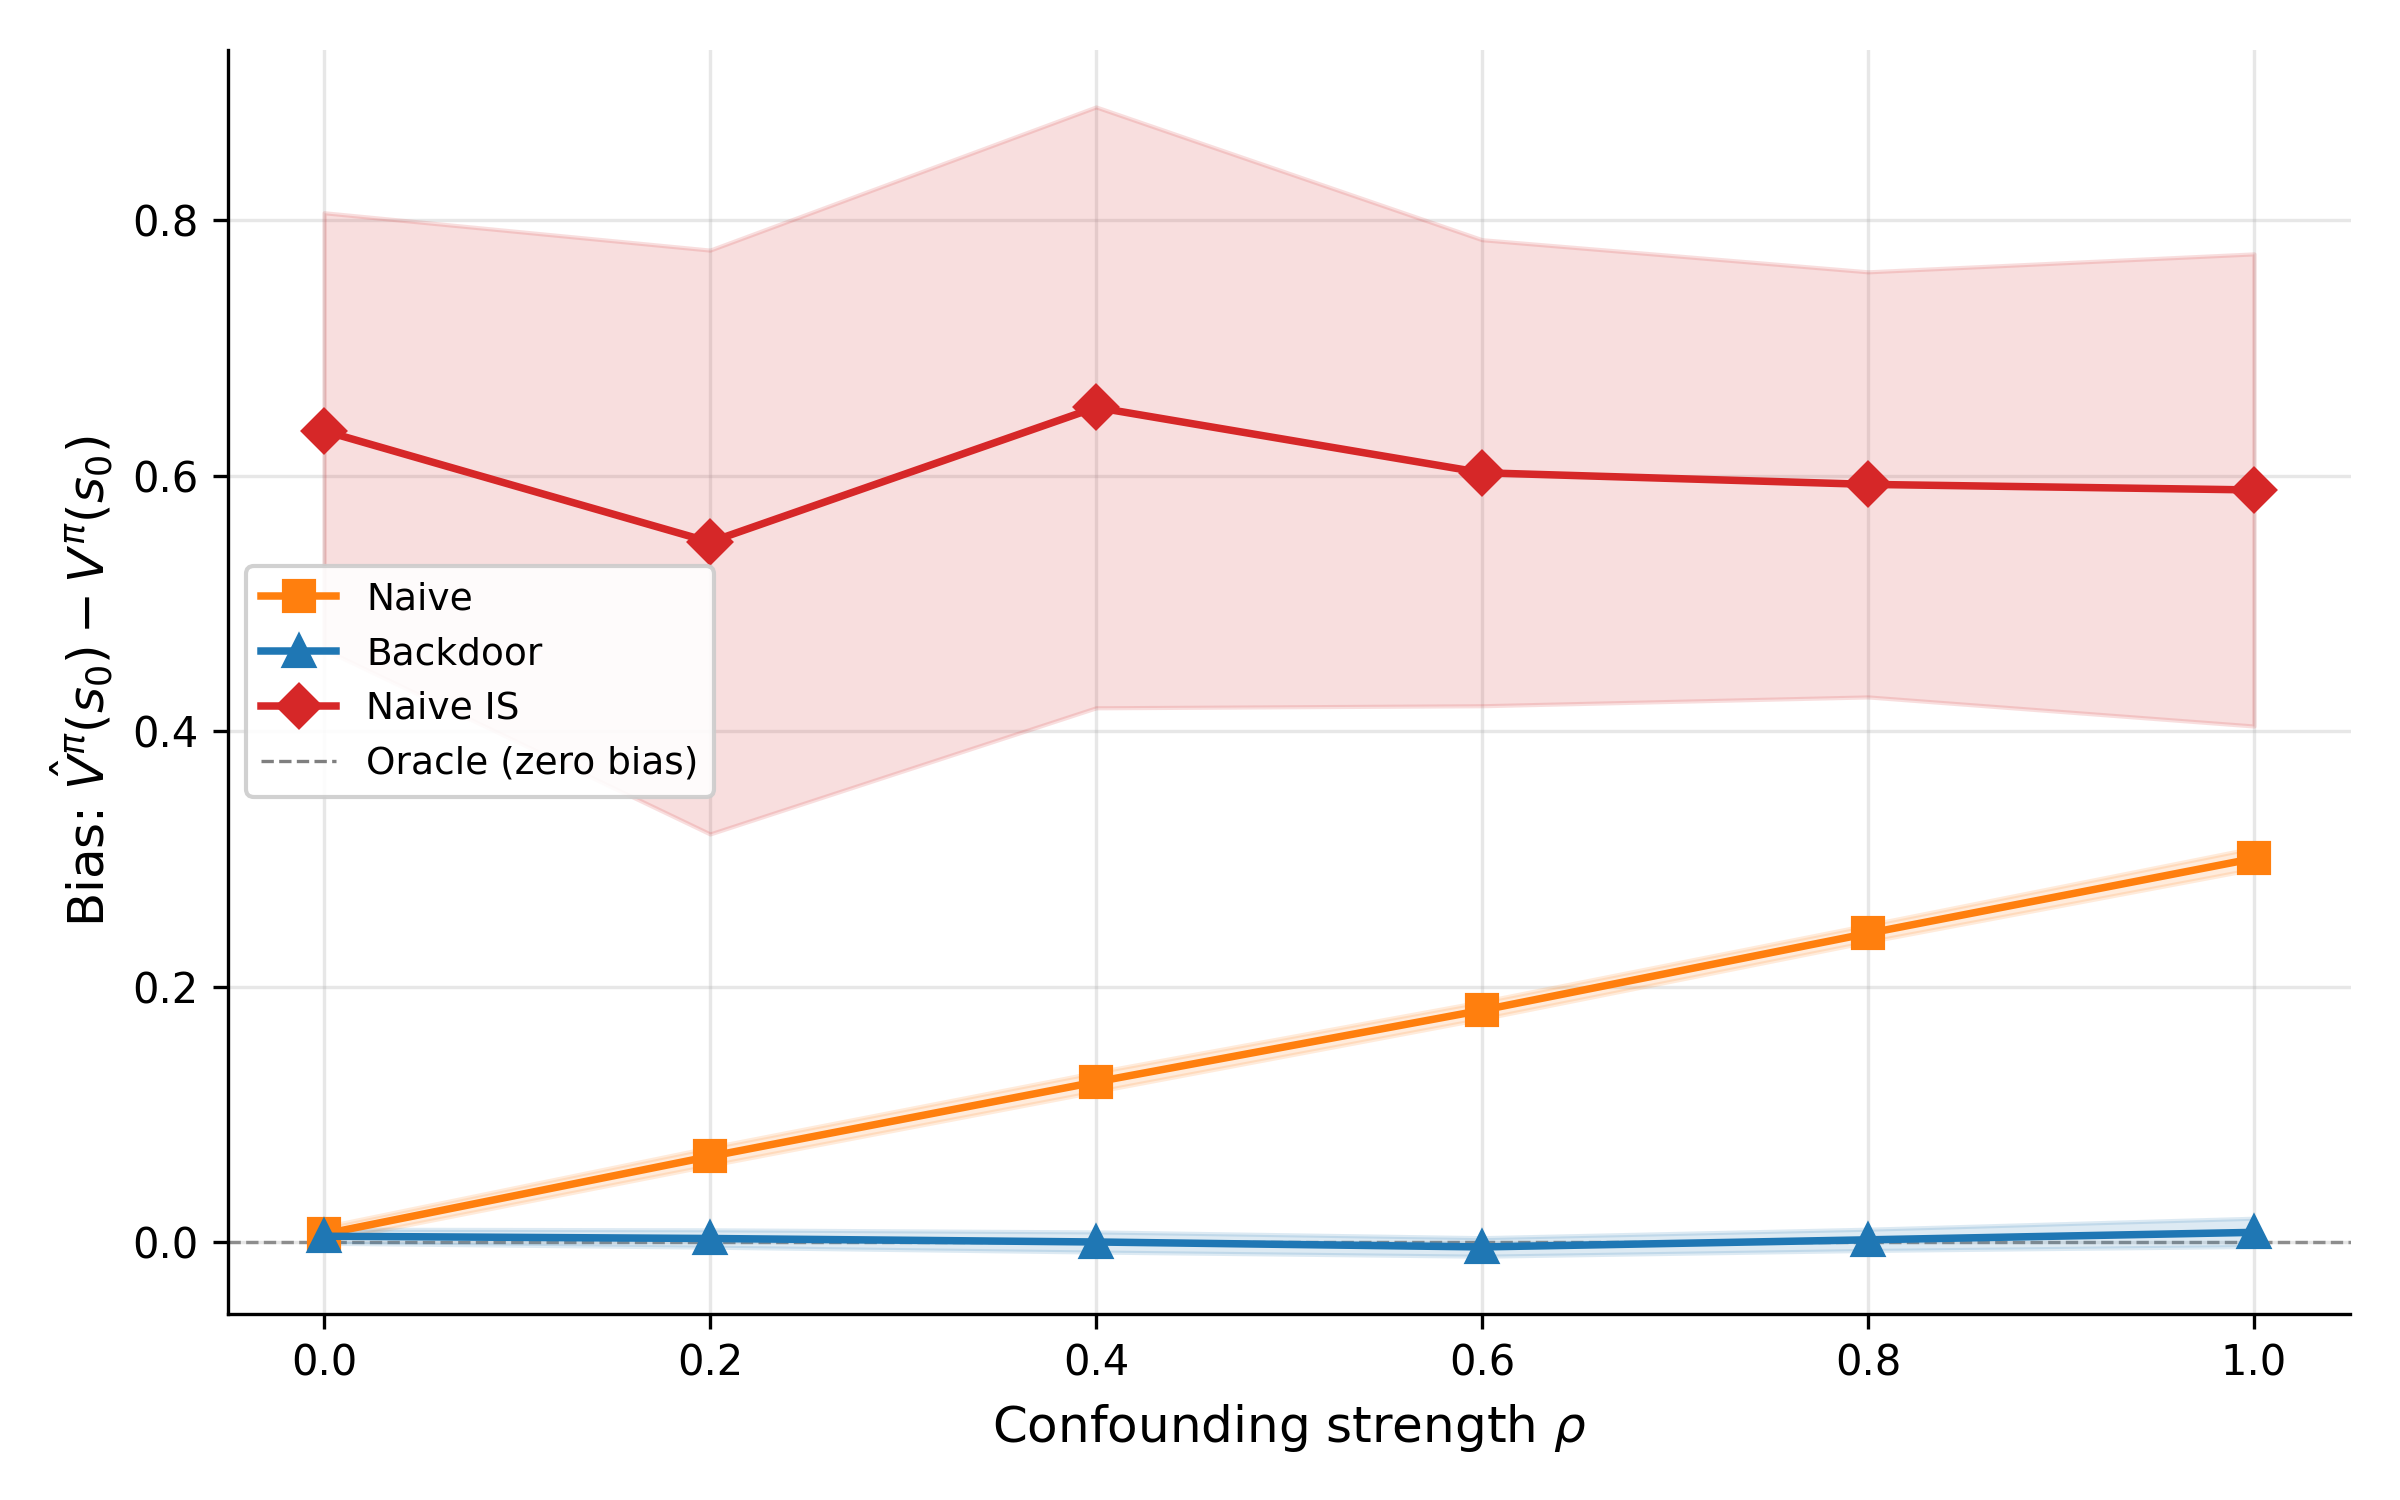
\includegraphics[width=0.75\textwidth]{../ch09_causal/sims/confounded_ope_bias.png}
\caption{Bias of three OPE estimators relative to the oracle as a function of confounding strength $\rho$. Naive bias grows monotonically as the behavioral policy's dependence on the unobserved confounder $U_t$ increasingly distorts observational transition estimates. The backdoor-adjusted estimator (Theorem~\ref{thm:backdoor_mdp}) remains unbiased at all confounding levels.}
\label{fig:confounded_ope}
\end{figure}
